\section{Examples} \label{sec:Examples}
In this section we want to include the following examples:
\begin{itemize}
	\item 1D chain with a single vertex (the ``simplest" decorator graph, which we discussed in the previous section), with coupling constants as zero coupling constants isn't that exciting
	\item The 2D-cross in plane example, with coupling constants. This is similar to the decorator case (at least in the dispersion relation which is derived), but could be used to show off some numerical results.
	\item (Potentially): A graph lacking symmetries, which requires a numerical treatment to find the eigenvalues?
\end{itemize}

Throughout this section, we are concerned with determining the spectrum of the problem \tstk{this is a recall, so no number but link to the first instance of it being stated}
\begin{align*}
	-\grad_{\ddmes} u &= \omega^2 u, \quad\text{on } \ddom.
\end{align*}

\subsection{Cross in the Periodic Plane} \label{ssec:ExampleCrossInPlane}
\tstk{intro sentence that provides relevance once we decide on the order to present the examples in}
Consider the periodic graph defined as follows; for each $\bracs{n,m}\in\integers^2$ define
\begin{align*}
	v_1^{\bracs{n,m}} = \bracs{\recip{2},0} + \bracs{n,m}, 
	&\quad v_2^{\bracs{n,m}} = \bracs{0,\recip{2}} + \bracs{n,m}, \\
	v_3^{\bracs{n,m}} = \bracs{\recip{2},\recip{2}} + \bracs{n,m}. & \\
	I_{13}^{\bracs{n,m}} = \sqbracs{v_1^{\bracs{n,m}}, v_3^{\bracs{n,m}}},
	&\quad I_{23}^{\bracs{n,m}} = \sqbracs{v_2^{\bracs{n,m}}, v_3^{\bracs{n,m}}}, \\
	I_{31}^{\bracs{n,m}} = \sqbracs{v_3^{\bracs{n,m}}, v_1^{\bracs{n+1,m}}},
	&\quad I_{32}^{\bracs{n,m}} = \sqbracs{v_3^{\bracs{n,m}}, v_2^{\bracs{n,m+1}}}.
\end{align*}
Then with 
\begin{align*}
	\vertSet^* &= \clbracs{v_j^{\bracs{n,m}} \ \vert \ j\in\clbracs{1,2,3}, \bracs{n,m}\in\integers^2}, \\
	\edgeSet^* &= \clbracs{I_{jk}^{\bracs{n,m}} \ \vert \ j,k\in\clbracs{1,2,3}, \bracs{n,m}\in\integers^2},
\end{align*}
and coupling constants
\begin{align*}
	\alpha_3^{\bracs{n,m}} &= \alpha \in\reals, \\
	\alpha_j^{\bracs{n,m}} &= 0, \quad j\in\clbracs{1,2,4,5},
\end{align*}
$\graph^* = \bracs{\vertSet^*,\edgeSet^*}$ is an embedded, periodic graph in $\reals^2$.
It's period graph occupies $\sqbracs{0,1}^2$ and can be visualised in figure \ref{fig:Diagram_TFRGraph}; consisting of 5 (although due to the association at the edges, effectively 3) vertices and 4 edges.
\begin{figure}[b!]
	\centering
	\begin{subfigure}[t]{0.45\textwidth}
		\centering
		\includegraphics[height=4.5cm]{Diagram_TFRGraph.pdf}
		\caption{\label{fig:Diagram_TFRGraph} The period graph that we are considering. All edges have length $\recip{2}$, and the quasi-momentum on horizontal edges is $-\qm_1$ and on vertical edges is $-\qm_2$.}
	\end{subfigure}
	~
	\begin{subfigure}[t]{0.45\textwidth}
		\centering
		\includegraphics[height=4.5cm]{Diagram_TFRQuantumGraph.pdf}
		\caption{\label{fig:Diagram_TFRQuantumGraph} The quantum graph that appears in our example in section \ref{ssec:CrossInPlane}. Due to the identification of vertices on the boundary of the period graph, we are effectively dealing with a 3-vertex quantum graph.}
	\end{subfigure}
	\caption{\label{fig:5VertexCross} (\ref{fig:Diagram_TFRGraph}) The period cell of the graph $\graph^*$. (\ref{fig:Diagram_TFRQuantumGraph}) The equivalent quantum graph on which we pose \tstk{qg eqn ref}, retaining the lengths $l_{jk}$ and appropriate $\qm_{jk}$.}
\end{figure}
After associating the edges of the period graph, we obtain it's associated quantum graph $\graph=\bracs{\vertSet,\edgeSet}$ with $\vertSet=\clbracs{v_1,v_2,v_3}$, $\edgeSet=\clbracs{I_{13},I_{23},I_{31},I_{32}}$, and lengths
\begin{align*}
	l_{13} = l_{23} = l_{31} = l_{32} = \recip{2}.
\end{align*}
Given that all the edges of $\graph^*$ are parallel to the co-ordinate axes, it is also fairly easy to compute the values of $\qm_{jk}$ for each $I_{jk}\in E$ and a given $\qm=\bracs{\qm_1,\qm_2}\in[-\pi,\pi)^2$;
\begin{align*}
	\qm_{13} = \qm_{31} = -\qm_2, &\quad \qm_{23} = \qm_{32} = -\qm_1.
\end{align*}

We now look to determine the spectrum of the problem \tstk{var problem eqn ref}, which by the analysis of section \ref{sec:Analysis} we can do by determining the eigenvalues $\omega^2$ of the system \tstk{QG equation system}.
Furthermore we can use proposition \ref{prop:M-MatrixEntries} to write down the $M$-matrix as
\begin{align*}
	M_{\qm}\bracs{\omega} &=
	\begin{pmatrix}
		2\omega\cot\bracs{\frac{\omega}{2}} & 0 & -2\omega\csc\bracs{\frac{\omega}{2}}\cos\bracs{\frac{\qm_2}{2}} \\
		0 & 2\omega\cot\bracs{\frac{\omega}{2}} & -2\omega\csc\bracs{\frac{\omega}{2}}\cos\bracs{\frac{\qm_1}{2}} \\
		-2\omega\csc\bracs{\frac{\omega}{2}}\cos\bracs{\frac{\qm_2}{2}} & -2\omega\csc\bracs{\frac{\omega}{2}}\cos\bracs{\frac{\qm_1}{2}} & 4\omega\cot\bracs{\frac{\omega}{2}}
	\end{pmatrix}.
\end{align*}
At this point we have the option of solving for the spectrum numerically or analytically, however because we have such a small and symmetric problem we proceed analytically by solving $\mathrm{det}\bracs{ M_{\qm}\bracs{\omega} - A }=0$. \tstk{note: we might have $A$ depending on $\omega$ when $\alpha$ is non-zero, so maybe add this dependence in explicitly? Also, has $A$'s form been given at this point, if not define!?}
After some calculation,
\begin{align*}
	\det\bracs{\bracs{M_{\qm}\bracs{\omega^2} - \omega^2 A}} &= 0 \\
	\Leftrightarrow \cos\bracs{\frac{\qm_1+\qm_2}{2}}\cos\bracs{\frac{\qm_1-\qm_2}{2}} &= \cos\omega - \frac{\alpha\omega}{4}\sin\omega. \labelthis\label{eq:ExampleThickVertexSolution}
\end{align*}
For ease, we define
\begin{align*}
	\Xi\bracs{\omega, \wavenumber} := \cos\omega - \frac{\alpha\omega}{4}\sin\omega.
\end{align*}
The left hand side of \eqref{eq:ExampleThickVertexSolution} attains every value in the interval $\sqbracs{-1,1}$ over the range $\qm\in[-\pi,\pi)^2$, but the right hand side cannot be written as a function of $\omega$ alone.
So finding eigenvalues $\omega^2$ amounts to determining those $\omega$ for which
\begin{align} \label{eq:ExampleThickVertexDispExpr}
	-1 \leq \Xi\bracs{\omega} \leq 1.
\end{align}
One can visualise the curve $\Xi$ in figure \ref{fig:Scalar_ThickVertexDR}; one can observe that the points $\omega$ that satisfy \eqref{eq:ExampleThickVertexDispExpr} are divided into distinct ``spectral bands" which shrink as $\omega\rightarrow\infty$.
The value of $\alpha$ changes the shape of $\Xi$ which in turn will also effects the resulting eigenvalues and spectral bands \tstk{do we want to give the results which validate the emergence of spectral bands? CF TFR.}.
\begin{figure}[t]
	\centering
	\begin{subfigure}[t]{0.45\textwidth}
		\centering
		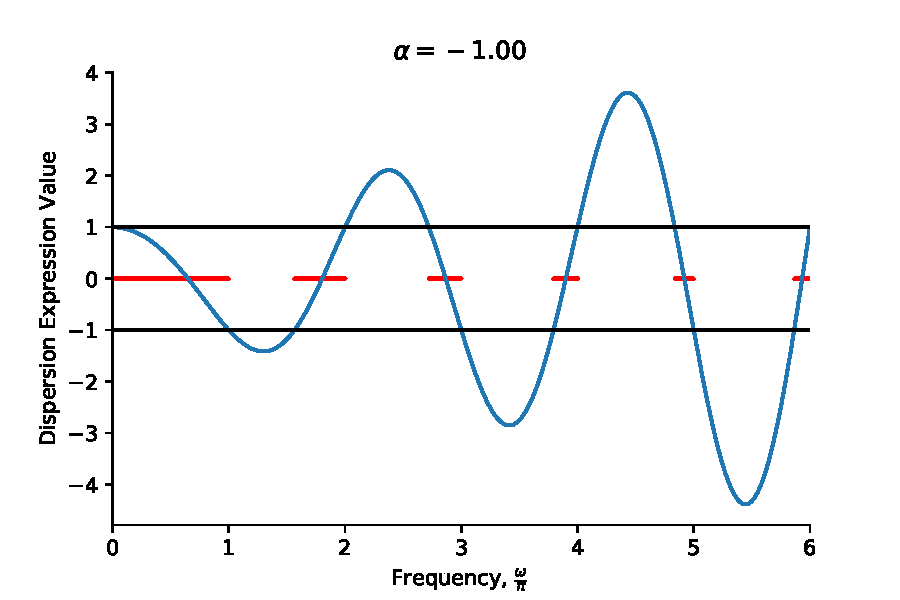
\includegraphics[scale=0.5]{Scalar_ThickVertexDR_a-1.pdf}
		\caption{\label{fig:Scalar_ThickVertexDR_a-1} The function $\Xi$ for $\alpha=-1$.}
	\end{subfigure}
	~
	\begin{subfigure}[t]{0.45\textwidth}
		\centering
		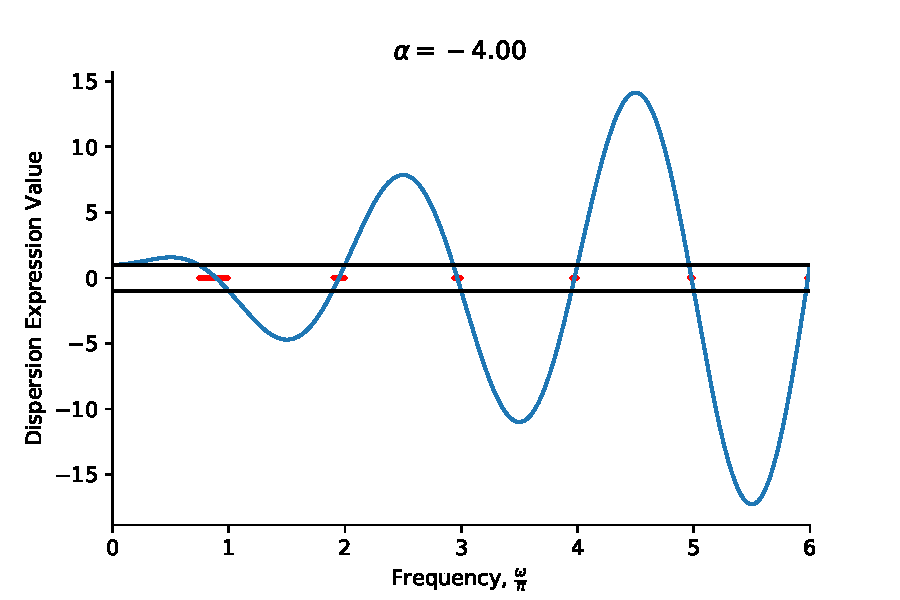
\includegraphics[scale=0.5]{Scalar_ThickVertexDR_a-4.pdf}
		\caption{\label{fig:Scalar_ThickVertexDR_a-4} The function $\Xi$ for $\alpha=-4$.}
	\end{subfigure}
	\caption{\label{fig:Scalar_ThickVertexDR} The function $\Xi$. Red regions indicate those $\omega$ that correspond to eigenvalues $\omega^2$, when $\Xi$ takes values between $-1$ and $1$ (black lines). One can see the existence of spectral bands which shrink in size as $\omega\rightarrow\infty$.}
\end{figure}
\tstk{also, we have a density of states now too, we could include that????}
